\begin{figure}
    \centering
    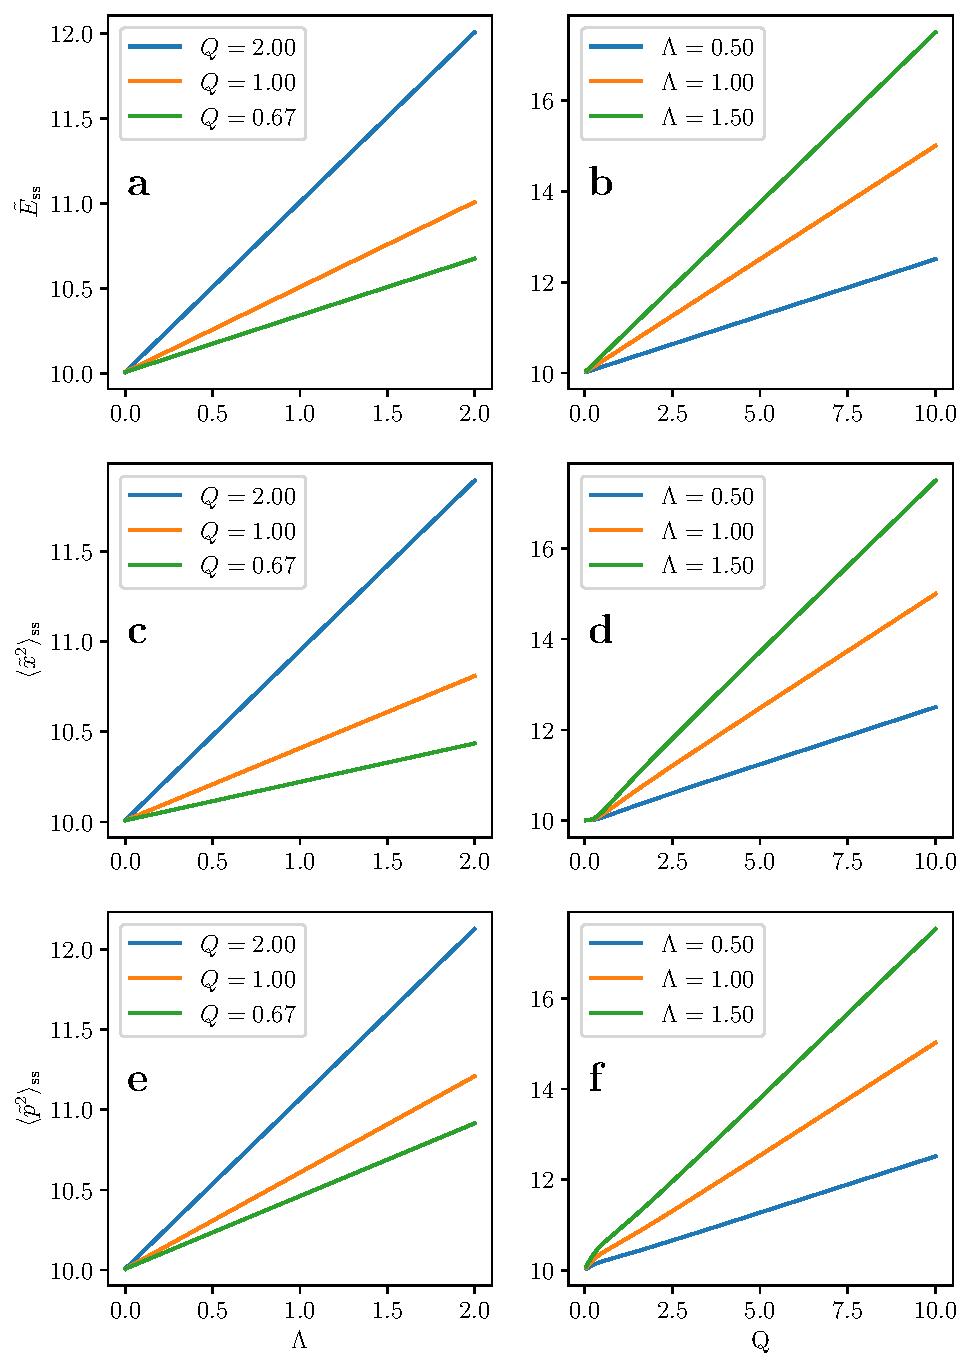
\includegraphics[width=\textwidth]{measurement_result.pdf}
    \caption{ \small The top panels show Eq. \eqref{eq:ess}, the middle panels show Eq. \eqref{eq:x2ss} and the bottom panels show Eq. \eqref{eq:p2ss}. All plots use the parameters $k_\mathrm{B}T = 10$ and $\omega = \hbar = 1$. The left panels are plotted against $\lambda / \omega$ and with three different values for $Q$, while the right panels are plotted against $Q$ and three different values of $\lambda$. }
    \label{fig:steady_state}
\end{figure}